\documentclass[11pt,a4paper]{article}
\usepackage[T1]{fontenc}
%\usepackage[latin1]{inputenc}
%\usepackage{amssymb,amsmath,a4wide}
\usepackage[utf8]{inputenc}
\usepackage{amssymb,amsmath}
\usepackage[pdftex]{graphicx}
\usepackage{ctable}
\usepackage{amsmath}
%\usepackage{threeparttable} %na
%\usepackage{tabu} %na
\usepackage{tabularx}
\usepackage{subfig}
\usepackage{rotating}
\usepackage{longtable}
%\usepackage[table]{xcolor} % clash with floatrow
\usepackage{xcolor} 
\usepackage{floatrow}
\usepackage{threeparttable}
%\usepackage[multiple]{footmisc} %na
\usepackage{bm}
\usepackage{fancybox}
%\usepackage{harvard}
\usepackage{geometry}         % Definir les marges
\geometry{verbose,a4paper,tmargin=1in,bmargin=1in,lmargin=1in,rmargin=1in}
\usepackage{setspace}
%\usepackage{ccaption}
\usepackage[colorlinks=true,citecolor=black, urlcolor=black, linkcolor=black]{hyperref}
\usepackage{url}
\newcommand{\email}[1]{\href{mailto:#1}{\nolinkurl{#1}}}
\usepackage[french, english]{babel}  % Placez ici une liste de langues, la derniere etant la langue principale
\usepackage{lscape}
\usepackage{afterpage}
\usepackage{supertabular}    %na            %  mettre pour les grands tableaux en formant paysage. marche avec \begin{landscape}
% style de la biblio : necessaire pour utiliser BibTex, necessite le deuxieme fichier exemple.bib
\usepackage{caption}
%\usepackage[longnamesfirst]{natbib}
\usepackage{natbib}
\bibliographystyle{elsarticle-harv}
\newcommand{\tqdl}{\textquotedblleft}
\newcommand{\tqdr}{\textquotedblright}
\linespread{1.2}
\begin{document}
\title{Global value chains and the transmission of price shocks\\
\vspace{1cm}
\normalsize{First draft version}
}
\vspace{1cm}
\date{\today}
\author{Marion Cochard\thanks{Banque de France, Sciences Po, OFCE. E-mail: \email{marion.cochard@banque-france.fr}}\and Guillaume Daudin\thanks{PSL, Universit\'e Paris-Dauphine,Sciences Po, OFCE. E-mail: \email{gdaudin@mac.com}}\and Violaine Faubert\thanks{Banque de France. E-mail: \email{violaine.faubert@banque-france.fr}} \and Antoine Lalliard\thanks{Banque de France. E-mail: \email{antoine.lalliard@banque-france.fr}} \and Christine Rifflart\thanks{Sciences Po, OFCE. E-mail: \email{christine.rifflart@ofce.sciences-po.fr}}
}
%\vspace*{\fill}
\maketitle
\begin{abstract}
{\small \noindent
Firms' participation in global value chains strengthens cross-country linkages via trade in intermediate inputs. 
In this paper, we build on two sectoral world input-output datasets  to assess the role of global input-output linkages in the propagation of inflationary shocks in the international economy. 
 %à faire: productivity shocks More specifically, we study the role of global input-output linkages in transmitting oil prices shocks across economies.
We examine the increasing integration of the European economies since the adoption of the common currency and investigate whether the shortening of global value chains in the wake of the Great Recession has changed the propagation of global inflationary shocks. We provide evidence that, following an appreciation of the domestic currency, the direct effect of global inflationary shocks, i.e. the share of imported final and intermediate goods in domestic consumption, explains the bulk of the propagation of global shocks to domestic consumer prices. By contrast, we find a limited role for the additional transmission of lower domestic input prices to other sectors of the domestic economy and other countries occuring during subsequent production cycles. Finally, building on sectoral data, we examine which sectors experience higher spillovers from global inflationary shocks.
%We also contribute to the literature on global input-output linkages by assessing whether results are consistent across the different world input output databases available (WIOD and TiVA).
}

{\small \bigskip \noindent \emph{JEL Classification}\/: C67, E31, F42, F62\\}
{\small \noindent \emph{Keywords}\/: input-output linkages, spillovers, global value chains, cost-push inflation, euro area \\}
\end{abstract}

\section{Introduction}
Trade liberalization and lower transportation and communication costs facilitated the fragmentation of production beyond national borders. As a result, firms' participation in global value chains strengthens cross-country linkages via trade in intermediate inputs. 
In the presence of imported intermediate goods, fluctuations in the prices of imports that are themselves driven by exchange rate movements affect the domestic cost of production and, ultimately, domestic consumer prices. 
As global value chains contribute to explaining the transmission of macroeconomic shocks across countries, a better understanding of trade spillovers has become paramount.  
In this paper, we build on the World Input-Output tables (WIOT hereafter) to investigate how production linkages give rise to nominal spillovers. 
We examine the extent to which domestic consumer prices react to changes in imported intermediate and final goods.
We pay particular attention to euro area countries, which have been increasingly participating in cross-border production chains following the adoption of the common currency. The euro area is indeed more involved in global production chains than other large economies, such as the United States and China \citep{ECB2016} and has been less affected by global value chains shortening than other countries in the years following the Great Recession. 
Building on sectoral data from the World InputOutput Database, we examine which sectors experience higher spillovers from global inflationary shocks.\\
To preview our findings, we find that...\\
The remainder of the paper is organized as follows. Section \ref{sec:lit} briefly describes the related literature. Section \ref{sec:metho} presents the methodology and the data sources.  Section \ref{sec:prixconso} presents the impact of an exchange rate shock on consumer prices.  Section \ref{sec:prixconsosecteur} examines which of the subcomponents of consumer prices experience higher spillovers from global inflationary shocks.
Section \ref{sec:ccl} provides some concluding remarks and avenues for future research.

\label{sec:intro}


\section{Related literature}
\label{sec:lit}
A recent literature examines whether trade in intermediate inputs is an important source of inflation synchronization across countries.
\cite{Auer2017} document that the cross-border propagation of cost shocks through input-output
linkages contributes substantially to synchronizing producer price inflation across countries, combining data on sectoral domestic and international input trade from the World Input Output
Database (WIOD) and producer price indices. By contrast, exchange rate movements and the degree of pricing-to-market are found to play no role in synchronizing inflation across countries.
\cite{AntoundeAlmeida2016} show that the cross-border sectors pairs which trade more intensively with each other in intermediate inputs display higher PPI inflation correlation, indicating  price spillovers along the global supply chain.\\
Our research is also related to the literature on exchange rate pass-through, in particular in an environment where intermediate inputs account for a large share of imports. For instance,  \cite{Goldberg2010} show that imported intermediate inputs are the dominant channel through wich changes in import prices pass to CPI inflation.\\
We improve on the literature on various respects. First, while most of the literature focusses on production prices, we examine the role of input-output linkages in propagating shocks to consumer prices. 
Secondly, we analyze how sectoral inflation reacts to global inflationnary shocks by examining the main components of consumer prices (manufacturing goods, services, food and energy).  We draw on the World Input-Output Database to examine which sectors experience higher spillovers from global inflationary shocks.
Thirdly, we provide evidence that, following an appreciation of the domestic currency, the direct effect of global inflationary shocks, i.e. the share of imported final and intermediate goods in domestic consumption, explains the bulk of the propagation of global shocks to domestic prices. By contrast, we find a limited role for the additional transmission of lower domestic input prices to other sectors of the domestic economy and other countries occuring during subsequent production cycles.
% à voir si on le fait: We assess whether results are robust to the use of different databases (WIOD versus OECD-ICIO). 

\section{Methodology }
\label{sec:metho}

\subsection{The Input-Output model applied to a shock on production costs.}
\label{subsec:io}
The widely known Leontief's production model (or I-O model) breaks down the impact of a demand shock \citep{Leontief1951}. The trade in value-added analysis reconciles international trade statistics with national I-O tables, which allows Leontief's analysis to be extended to an international context. A number of studies \citep{Hummels2001,Daudin2006,Daudin2011, DeBacker2012,Johnson2012,Koopman2014, Amador2015,Los2016} analyze the value added content of world trade. Some authors focus on Asia \citep{Sato2014} or on the euro area \citep{Cappariello2015}. \cite{Bems2015} focus on competitiveness and compute real effective exchange rates weighted by the value-added trade structure to measure the impact of a change in relative prices on each country's value added.
Leontief's production model has a dual: the price model. Some studies focus on the consequences of a change in production prices based on an I-O model or a SAM (Social Accounting Matrix) model in developing countries. Leontief's price model is broadly used in multi-sector, single-country macroeconomic models, for example, to measure the effect of a change in energy prices \citep{Bournay2015, Sharify2013}. To the best of our knowledge, the dual production model of Leontief has only been adapted in an international context \cite{Cochard2016}. 
This is an accounting approach to the effect of costs on prices ("cost-push inflation"). Firms' margins are assumed to be fixed. Prices only adjust to absorb cost changes, production techniques are fixed during successive production cycles and inputs substitution (for instance, between countries producing the same goods) is not accounted for, despite variations in relative price. The limitations of this approach are well known \citep{Folloni1994}. In particular, and although the division of global value chains largely takes place within multinational firms, it considers a unique pricing system based on market prices and independent of firm strategies. Still, this method provides a measure of the vulnerability of each sector to price or productivity shocks \citep{Acemoglu2012,Carvalho2014}. Hence, though unrealistic, it is useful for identifying which countries and sectors are under pressure to adjust their prices when subject to exogenous cost shocks. For instance, it can show which euro area countries benefited most from an appreciation of the euro or whether adopting the euro has increased interdependence between member countries.


\subsection{Applying the I-O model to a price model}
\label{subsec:ioprice}
The standard I-O model relies on input-output tables registering transactions of goods and services (domestic or imported) at current prices. I-O tables describe the sale and purchase relationships between producers and consumers within an economy. Each column describes, for each industry $j$, the intermediate consumption of goods and services from the various sectors. Each column indicates the payment of intermediate consumption and the remuneration of production factors. By construction, the I-O tables are balanced: the sum of resources equals the sum of expenditures for the whole economy. The rows of the table contain information on the distribution of the output of industries over use categories.
Define $Y$ the vector of production of dimension $(1, n)$, $A$ the matrix of input coefficients of dimension $(n, n)$, and $R$ the vector of factor incomes of dimension $(1, n)$.\\
\begin{eqnarray*}
	Y=(y_1\ldots y_n)=\left(y_1\ldots y_n\right)\left( \begin{matrix}
   a_{11} & \cdots  & a_{n1}  \\
   \vdots  & a_{ij} & \vdots   \\
   a_{1n} & \cdots  & a_{nn}  \\
\end{matrix} \right)+(r_1\ldots r_n)=YA+R
\end{eqnarray*}
Assuming that there is no possible substitution between inputs (i.e. that technical coefficients are fixed), we can derive a price equation under the assumption of complete cost pass-through.\\
Define $y_i=p_i*q_i$, with $p_i$ the price and $q_i$ the quantity of product $i$ and normalize quantity such as $q_i=1$. \\
Define $A$ the structural matrix of the technical coefficients of dimension $(n, n)$, $P$ the vector of production prices of dimension $(1, n)$ and $V$ the vector of factor income of dimension $(1, n)$. Then $P=PA+V$. \\
When an exogenous input price shock occurs, firms face a change in their costs, which is passed on directly to production prices. This exogenous shock is assumed not to affect the return on capital and labor. Therefore, there is no adjustment to margins. Under these conditions, for each industry $i$, the shock can be written as the absolute difference between the initial production price and the new production price invoiced following the shock ("shocked price" hereafter).\\
Define ${{\Delta }^{0}}P$ the shock vector of dimension $(1, n)$ computed as the difference between the original price $P^0$ and the vector $P^1$ of shocked prices. Then:
\begin{eqnarray*}
\Delta ^{0}P=P^1-P^0=c, 
\end{eqnarray*}
with $c$ the shock vector of dimension (1,n), which contains the direct effect of the shock on output prices.\\
The price increase is passed on to the industries that use shocked products as intermediate consumptions. The higher the reliance on shocked inputs, the higher the increase in production prices.\\
In a first step, the direct impact of the shock on each industry's output prices amounts to $\Delta^{1}P=cA$.\\
In a second step, the shock is passed on all industries using these shocked inputs in their production processes. For $n$ production cycles, the increase in production prices amount to $\Delta^n P=cA^n$.\\
As the technical coefficients are smaller than 1, the effect of the initial shock on input prices eventually wears out. Finally, the overall effect of the shock is equal to the sum of the initial shock and all the increases that occurred during the successive production cycles. The total effect of the shock on prices, S, is equal to $S=c \!\!~\!\!\text{ }{{\left( I-A \right)}^{-1}}$, with $\text{ }\!\!~\!\!\text{ }{{\left( I-A \right)}^{-1}}$ the inverse of Leontief's matrix; $S$ is a vector $(1, n)$ composed of the elements $s_{ij}$ measuring the total effect of the shock on the output price of country $i$'s sector $j$ and $C~$ is the vector of an exogenous input price shock.\\
To compute which countries are most affected by a production cost shock through value-added and vertical trade flows in international trade, we need a large structural matrix that integrates input flows between sectors within each country and between countries. This matrix traces the sectoral and geographical origin of inputs produced worldwide. On the diagonal are the country blocks with flows of domestic transactions of intermediate goods and services between industries. The country blocks outside the diagonal represent international flows of intermediate goods and services via bilateral sectoral exports and imports. 


\subsection{Data and measurement issues}
\label{subsec:data}

The world input-output table is an extension of the national input-output tables. Input-output tables measure the relationships between the producers of goods and services (including imports) within an economy and the users of these goods and services (including exports). Hence, the national tables specify, for each industry, the use of the product, being for either intermediate or final use. The latter includes domestic final use (consumption and investment) and exports. The world input-output table shows in which foreign industry a product was produced, and which foreign industry or final user uses the exports of a given country. Hence, world input-output tables enable us to identify how much international trade is associated with the consumption of a particular final product. \\
The use of national input-output tables as part of a global framework is challenging for two reasons. First, national input-output tables vary widely in terms of detail and scope, and are therefore not fully consistent. Second, the availability of national input-output tables for a is limited, especially for developing economies. 
Two sectoral datasets for international intput-output tables are available: (\textit{i}) the World Input Output Database (WIOD) and (\textit{ii}) the OECD-ICIO database TiVA.
\paragraph{The World Input Output Database (WIOD)}
The World Input Output Database (WIOD) contains time series of inter-country input-output tables from 2000 to 2014.  World Input-Output tables (WIOT) connect national tables with international trade flows. WIOD uses supply-use tables (SUT) from individual country's national accounts as the starting point to integrate with bilateral trade statistics and derive the final symmetric WIOT. The WIOD covers 43 countries, of which a majority belongs to the European Union, as well as the rest of the world, constructed as one economy. 
These global Input-Output (I-O thereafter) tables encompass major advanced and emerging countries and cover around 85$\%$ of world GDP. They contain annual information for 56 industries, comprising primary, manufacturing goods and services sectors. Therefore, for each year a full country-sector input-output matrix traces the importance of a supplying industry in one country for an industry in another country. The values in WIOTs are expressed in millions of U.S. dollars; market exchange rates were used for currency conversion \citep{TimmerIllustratedUserGuide2015}. % All transactions values are in basic prices, reflecting all costs borne by the producer. These tables are accompanied by Socio-Economic Accounts which contain country sector panel data on employment (number of workers, compensation and share of labor in high, medium and low skilled occupations), capital stocks, gross output and value added).
Table \ref{tab:wiod} shows the economies included in the WIOD.
 
 
\begin{table}[!h]
\begin{threeparttable}
\centering
\centering
\caption{\small{\textbf{Economies included in the World Input-Output Database}}}
\small
\begin{tabular}{ll}
\hline\hline
Europe & Austria, Belgium, Bulgaria, Croatia, Cyprus, Czech Republic, Denmark,\\
& Estonia, Finland, France, Germany, Greece, Hungary, Ireland, Italy,\\
& Latvia, Lithuania, Luxembourg, Malta, Netherlands, Norway, Poland,\\
&Portugal, Romania, Slovakia, Slovenia, Spain, Sweden, Switzerland,\\
& United Kingdom\\
North  America& Canada, United States\\
Latin America & Brazil, Mexico \\
Asia-Pacific & Australia, China, India, Indonesia, Japan, Korea, Taiwan\\
Other & Russia, Turkey\\
\hline\hline
\end{tabular} 
\label{tab:wiod}
\end{threeparttable}
\end{table} 

\paragraph{The Statistics on Trade in Value Added (TiVA) database}
The TiVA database is compiled by the OECD and the WTO. It builds on the OECD harmonized individual country I-O tables to provide matrices of inter-industrial flows of goods and services in current prices (USD million), for 64 economies (i.e. 35 OECD Countries, 28 non-OECD economies and the Rest of the world) and 34 industries, covering the years 1995 to 2011. 
Table \ref{tab:tiva} shows the economies included in the TiVA database.

\begin{table}[!h]
\begin{threeparttable}
\centering
\centering
\caption{\small{\textbf{Economies included in the TiVA Database}}}
\small
\begin{tabular}{ll}
\hline\hline
Europe & Austria, Belgium, Bulgaria, Croatia, Cyprus, Czech Republic, Denmark,\\
& Estonia, Finland, France, Germany, Greece, Hungary, Iceland, Ireland, Italy,\\
& Latvia, Lithuania, Luxembourg, Malta, Netherlands, Norway, Poland,\\
&Portugal, Romania, Slovakia, Slovenia, Spain, Sweden, Switzerland,\\
& United Kingdom\\
North  America& Canada, United States\\
Latin America & Argentina, Brazil, Chile, Colombia, Costa Rica, Mexico, Peru\\
Asia-Pacific & Australia, Cambodia, China, Hong Kong SAR, India, Indonesia, Japan, Korea,\\ &Malaysia, New Zealand, Philippines, Singapore, Taiwan, Thailand, Viet Nam\\
Other & Brunei, Israel, Morocco, Russia, Saudi Arabia, South Africa, Tunisia, Turkey\\
\hline\hline
\end{tabular} 
\label{tab:tiva}
\end{threeparttable}
\end{table} 


\paragraph{Major differences between the WIOD and TiVA databases}
The WIOD and TiVA databases have a number of distinguishing characteristics (see \cite{Timmer2015} for details). The difference most relevant for our analysis relates to the treatment of imports by use category. From national input-output statistics one can derive the use of products by industries and final consumers, but the country of origin of these products is unknown. Therefore, one has to breakdown product import statistics by category of use in the construction of WIOTs.\\
The TiVA database relies on the so-called import proportionality assumption. The domestic I-O tables show transactions between domestic industries. As a complement to these tables, supplementary tables break down total imports by user (industry and the different categories of final demand). Some countries provide these import tables in conjunction with their I-O tables, but in other cases they are derived by the OECD. The main assumption used in creating these import matrices is the proportionality assumption, which assumes that the share of imports in any product consumed directly as intermediate consumption or final demand (except exports) is the same for all end-uses  \footnote{See http://www.oecd.org/sti/ind/49894138.pdf for details.}.\\
Various studies have found that this assumption can be misleading, as import shares vary significantly across end-uses. \cite{Feenstra2012} find that shares of imported materials may differ substantially across U.S. industries. Based on Asian I-O tables, \cite{Puzzello2012} finds that the use of the standard proportionality assumption understates the use of foreign intermediate inputs. Hence, the import proportionality assumption is likely to be particularly binding for developing countries, as the import content of exports is usually higher than the import content of products destined for domestic consumption.\\
To address this issue, the WIOD database uses bilateral trade statistics to derive import shares for three end-use categories (intermediate use, final consumption and investment) by mapping detailed six-digit products based on extensive product description \citep{Dietzenbacher2013}.\\
To sum up, the WIOD includes information on bilateral industry-specific input use, whereas such information exists only in imputed form in TiVA. Therefore, we focus on the WIOD database in our analysis \footnote{Results obtained with the TiVA database are available on request.}. 


\subsection{Nominal exchange rate shock}
\label{subsec:chocchange}

We implement an exchange rate shock on the WIOT databases described above. 
The appreciation of a currency against other currencies leads, for the shock-stricken country, to a fall in the domestic-currency price of its imports and an increase in the foreign-currency price of its exports. We measure the disinflationary impact of this shock on the shock-stricken country and, conversely, its inflationary impact on countries that directly and indirectly consume, through third countries linkages, inputs from the shock-stricken country.\\
Suppose a world with two countries A and B, each having its own national currency, and a currency for international transactions, the dollar. \\
Assuming a 100$\%$ appreciation of the currency of country $A$ against the other two currencies, the production prices of country $A$ expressed in dollars would double compared to those of country $B$ expressed in dollars. Country $B$ pays more for its imports of inputs, in dollars as well as in national currency, since the exchange rate of the currency of Country $B$ against the dollar has not changed. Conversely, the imported input prices in country $A$ remain constant in dollar terms, since production prices of country $B$ have not changed and fall by half once expressed in national currency.\\
We assume that producers have no margin behavior and pass through the exchange rate shock fully on to their production prices. The change in the prices of imported goods is therefore transmitted to all domestic prices, both directly and through inter-industry linkages. These upward (downward) movements for country $B$ (country $A$), affect all input prices in each of the countries.\\
The effects of the shock spread over multiple production cycles. At the end of this process, the overall impact of the shock in dollar terms is equal, for the shocked country $A$, to the rise in production prices due to the exchange rate shock, minus direct and indirect decreases (via interindustry linkages in the country), in national currency and then converted back into dollar terms, in the prices of inputs imported from $B$ and disseminated to all branches. The overall impact on production prices in dollar terms in country $A$ is therefore lower than the initial exchange rate shock. For country $B$, the final impact is to the cumulative direct and indirect effects of higher prices of inputs imported from country $A$ and disseminated to all industries.\\
In a global economy composed of $P$ countries, each with $n$ sectors, the appreciation of a country's currency $i$ against all other currencies translates into a rise in the common currency, the dollar for example, in its relative prices vis-\`a-vis the rest of the world. \\ 
The production prices of each sector will vary in dollar terms from:
\begin{eqnarray*}
c_{\$1}=c_{\$2}=\ldots=c_{\$n}=c_{\$i} 
  \end{eqnarray*}	
in the shock-stricken country$~i$ and 0 in other countries. \\
Hence, for each sector $j$ in country  :
\begin{eqnarray*}
 {{\Delta }^{0}}p_{\${ij}}=p_{\${ij}}^{1}-p_{\${ij}}^{0}=c_{\${ij}}=c_{\${i}}
  \end{eqnarray*}	
And for any country $k$ different from $i$,
\begin{eqnarray*}
 {{\Delta }^{0}}p_{\${kj}}=p_{\${kj}}^{1}-p_{\${kj}}^{0}=c_{\${kj}}=0
 \end{eqnarray*}	
To simplify, output prices for each sector are normalized to 1 and exchange rates to 1:1. A 100$\%$ appreciation in the exchange rate of a currency against other currencies therefore corresponds to an absolute shock of +1, with production prices in the shock-stricken country rising from 1 to 2 dollars. The appreciation affects producers through changes in relative prices between countries and, therefore, through changes in input prices traded between the shock-stricken country $i$ and other countries. \\
Consider first the direct impact (in absolute terms) on other countries of the rise in imported input prices from shocked country $i$. For any sector l of a country $k$ ($k\ne i)$, the increase in the producer price depends directly on the quantity of inputs imported from the shock-stricken country $i$, weighted by the variation in level of the price of inputs in dollars (i. e. the exchange rate shock):\\
\begin{eqnarray}
\Delta ^1 p_{\${kl}}=c_{\${i}}*a_{kl}a_{i1}+\ldots+c_{\${i}}*a_{kl}a_{ij}+\ldots+c_{\$i}*a_{kl}a_{in}=\underset{j=1}{\overset{n}{\mathop\sum}}\,{c}_{\$i}*a_{kl}a_{ij}=c_{\$i}*\underset{j=1}{\overset{\text{n}}{\mathop\sum}}\,a_{kl}a_{ij}  
\label{eq:eq1} 
\end{eqnarray}
With $a_{kl}a_{ij}$ the quantity of inputs from the country's sector needed to develop a production unit for the country's $k$ sector $l$. \\
For the shocked country, the shock has a disinflationary effect on domestic production prices. In national currency, the production prices of imported inputs fall by $\widetilde{c_i}=-\frac{c_{\$i}}{1+{c_{\$i}}}$, or by 0.5 with $c_{\$i}=1$. \\
This decline is spread to all sectors during the production cycle. In sector $j$ of the shocked country $i$, this fall amounts in national currency to: \\
\begin{eqnarray*}
\Delta^1p_{ij}=\underset{l=1}{\overset{l=n}{\mathop \sum}}\,{\tilde{c}_{i}}*a_{ij}a_{1l}+\ldots +\underset{l=1}{\overset{{l}=n}{\mathop \sum }}\,{{\tilde{c}}_i}*a_{ij}a_{kl}+\underset{l=1}{\overset{l={n}}{\mathop \sum }}\,{{{\tilde{c}}}_{i}}*{{a}_{{ij}}}{{{a}}_{pl}}=\left( -\frac{{{c}_{\$i}}}{1+c_{\$i}}\right)*\underset{\begin{matrix}k=1\\k\neq i\\\end{matrix}}{\overset{{k}={p}}{\mathop\sum}}\,\left[\underset{l=1}{\overset{l=n}{\mathop\sum}}\,a_{ij}a_{kl}\right] 
\end{eqnarray*}
This level shock can be converted into dollars: \\
\begin{eqnarray}
{{\Delta }^{1}}{{{p}}_{\$ij}}=\left(1+{{c}_{\$i}}\right)*\left(-\frac{{{{c}}_{\$i}}}{1+{{{c}}_{\$i}}}\right)\underset{\begin{matrix}k=1\\k\neq i\\\end{matrix}}{\overset{{k}={p}}{\mathop\sum}}\,\left[\underset{\text{l}=1}{\overset{{l}={n}}{\mathop\sum}}\,{{{a}}_{\text{ij}}}{{{a}}_{{kl}}}\right] 
\label{eq:eq2}
\end{eqnarray}
We therefore know the direct impact of the shock on all input prices of all countries.
In matrix notation, we create two matrices that build on the large matrix $A$. These two matrices retain only the direct effects of the exchange rate shock on the price of goods imported by the shocked country $i$ and the direct effects of the exchange rate shock on the price of goods imported by the rest of the world from the shocked country $i$. To formalize the initial impact of the shock on the price of traded goods, we neutralize the impact of an input price shock on the price of domestic inputs as well as on the price of inputs traded between countries that are not shocked.\\
Let us first look at the shock from the perspective of countries that import inputs from country $i$.\\
Let ${{c}_{\$}}$ be the vector of change in production prices in dollars following the 100$\%$ appreciation of the currency of country $i~$ against all other currencies, corresponding to an absolute shock of $+1$ dollar for all sectors in country $i$. \\
Hence,
\begin{eqnarray*}
 c_\$=\left(0\ldots0\ldots c_{\$ij}\ldots c_{\$ik} 0\ldots0\right)
\end{eqnarray*}
with $c_{\$ij}=c_{\$ik}=c_{\$i}=1$
for all sectors $j$ and $k$ in the shocked country $i$.\\
Building on Equation \ref{eq:eq1}, we write the direct impact of the exchange rate shock on the other countries as the product of the shock vector $c_{\$}$ and a matrix $B$. $B$ builds on the large matrix $A$ of technical coefficients, but only keeps the coefficients of each country's sectoral inputs imported from the shocked country $i$. The other coefficients are replaced by 0, including those of the block of country $i$ concerning the domestic inputs of the shocked country $i$. The direct impact of the appreciation of a currency against the dollar on the price of inputs is equal to $c_{\$}B$ with
\begin{eqnarray}
{c_{\$}}B=\left(0\ldots c_{\$i}\ldots 0\right)\left(\begin{matrix}0&\cdots&0\\a_{1l}a_{ij}&0&a_{nl}a_{ij}\\0&\cdots&0\\\end{matrix}\right) 	
\label{eq:eq3}
\end{eqnarray}
where each ${{{a}}_{{kl}}}{{{a}}_{{ij}}}$ element of the line block represents the technical coefficient related to imports of inputs by sector $l$ in country $k$ (with $k~\ne ~i$) from sector $j$ in country $i$.\\
Let us now consider the shock from the perspective of the shocked country $i$.\\
Define ${{\tilde{c}}_{\$}}$ the vector of change in input prices imported by country i, in dollars, $( -c_{\$i}\ldots0\ldots-c_{\$i})$. \\
From Equation \ref{eq:eq2}, we can write the direct impact for country $i$ of the fall in input prices from the rest of the world. The direct impact corresponds to the product of the shock vector ${\tilde{c}}$  and a matrix ${\tilde{B}}$. ${\tilde{B}}$ builds on the large matrix A of which only the country blocks of the inputs imported by country $i$ from other countries have been retained. The other coefficients are replaced by 0, including those of the block of country $i$ concerning the domestic inputs of the shocked country $i$. \\
The direct impact of the appreciation of the shocked country $i$ on the price of its inputs corresponds, in dollars, to ${{\tilde{c}}_{\$}}{\tilde{B}}$ with: 
\begin{eqnarray}
{{\tilde{c}}_{\$}}{\tilde{B}}=\left(-{{{c}}_{\$i}}\ldots0\ldots-{{{c}}_{\$i}}\right)\left(\begin{matrix}0&\ldots{{{a}}_{{i}1}}{{{a}}_{11}}\ldots&0\\0&0&0\\0&\ldots{{\text{a}}_{\text{il}}}{{{a}}_{{pn}}}\ldots&0\\\end{matrix}\right) 
\label{eq:eq4}
 \end{eqnarray}
where each ${{{a}}_{{ij}}}{{{a}}_{{kl}}}$ element in the column block represents imports of inputs by sector $j$ in country $i~$from sector$~l$ in country $k$.
The direct effect on the world is therefore the sum of these vectors from equations  \ref{eq:eq3} and \ref{eq:eq4}, i. e. ${{c}_{\$}}{B}+{{\tilde{c}}_{\$}}{\tilde{B}}.~$\\
An input price shock then spreads to all sectors in all countries via the global intersectoral exchanges transcribed by the matrix of technical coefficients of the large matrix A. This process will be repeated several times, until the effects are completely exhausted.
In the end, the total effect of the dollar shock is equal to the shock itself, incremented by changes in input prices due to changes in imported input prices, and by all marginal changes in output prices during the production processes, i. e.:\\
\begin{eqnarray*}
	S_\$=\Delta{{P}_{\$}}=c_{\$}+(c_{\$}B+{{{\tilde{c}}}_{\$}}{\tilde{B}})+\left({{c}_{\$}}{B}+{{{\tilde{c}}}_{\$}}{\tilde{B}}\right){A}+\left({{c}_{\$}}{B}+{{{\tilde{c}}}_{\$}}{\tilde{B}}\right){{{A}}^{2}}+\ldots+\left({{c}_{\$}}{B}+{{{\tilde{c}}}_{\$}}{\tilde{B}}\right)A^n \\
 \end{eqnarray*}
 \begin{eqnarray}
{{S}_{\$}}={{c}_{\$}}+({{c}_{\$}}B+{{\tilde{c}}_{\$}}\tilde{B})*{{(I-A)}^{-1}}	
\label{eq:eq5}
 \end{eqnarray}
With ${{S}_{\$}}$ the total impact vector composed of the elements ${{{s}}_{\$ij}}$ showing the total impact of the shock on country $i$'s sector $j$. \\
Equation \ref{eq:eq5} gives the absolute evolution of input prices in international currency. To obtain the absolute evolution of the input prices of the shocked country in national currency, we remove the exchange rate shock and multiply this balance by the scalar of conversion equal to $\frac{1}{1+{{{c}}_{\$i}}}=0.5~$, since according to our hypotheses ${{{c}}_{\$i}}$=1:
\begin{eqnarray*}
	S=\left( \frac{1}{1+{{c}_{\$i}}}\right)*\left({{S}_{\$}}-{{c}_{\$}}\right)
\end{eqnarray*}
With $S$ a vector in shocked currency for all countries of the world. $S$ represents the overall impact of a shock on prices in each branch of each country. The average effect of the shock on output prices in each country $\bar{S}$ is computed as a weighted average of the sectoral effects of the shock. For each country, we compute a weighted average of the shock effects, based on three types of aggregation: the sectoral structure of output, the sectoral structure of exports and the sectoral structure of household consumption.\\
Hence 
\begin{eqnarray*}
\overline{s_{i}^{Y}}=\underset{j=1}{\overset{n}{\mathop \sum }}\,\frac{{{s}_{ij}}.{{y}_{ij}}}{{{y}_{i}}}
 \end{eqnarray*}
represents the average effect of the shock on output prices in country$~i$, with ${{{s}}_{{ij}}}$ the impact of the shock on the output prices of industry $j$ for country $i$, ${{{y}}_{{ij}}}$ the output of industry $j~$in country $i$ and ${{{y}}_{{i}}}$ the total output of country $i$. \\
This weighting scheme provides the impact of the shock on each country's production costs ("production prices" hereafter).\\
The second type of aggregation relies on the sectoral structure of exports. $\overline{s_{i}^{X}}$ provides the average impact of the shock on the export price competitiveness of country $i$. This export price indicator will be referred to as "export price" hereafter. \\
 \begin{eqnarray*}
\overline{s_{i}^{X}}=\underset{j=1}{\overset{n}{\mathop \sum }}\,\frac{{{s}_{ij}}.{{x}_{ij}}}{{{x}_{i}}},
 \end{eqnarray*} 
with $x_{ij}$the exports of industry $j$ in country $i$ and $x_{i}$ the total exports of country $i$. \\
The last type of aggregation relies on the sectoral structure of household consumption. Hence, $\overline{s_{i}^{HC}}$ provides the average impact of the shock on the consumer price of country $i$. 
 \begin{eqnarray}
\overline{s_{i}^{HC}}=\underset{j=1}{\overset{n}{\mathop \sum }}\,\frac{{{s}_{ij}}.h{{c}_{ij}}}{h{{c}_{i}}}
\label{eq:eq6}
 \end{eqnarray} 
with $hc_{ij}$ the consumption of industry $j$ in country $i$ and ${h}{{{c}}_{{i}}}$ the total household consumption of country $i$. 

\section{The impact of exchange rates fluctuations on consumer prices}
\label{sec:prixconso}


\subsection{The intensity of import in domestic consumption}
\label{subsec:intensity}
\begin{figure}[!h]
\centering
\caption{\footnotesize{\textbf{The share of imported intermediate and consumer goods in private consumption }}}
\begin{tabular}{c}
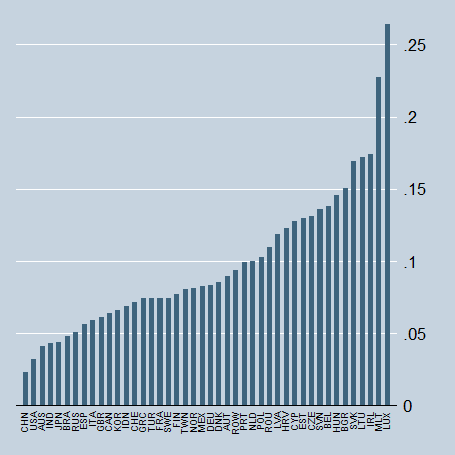
\includegraphics[width=5.0in, height=3.5in]{Graph_ratioimp_wiod_2014}\\
\floatfoot{Source: WIOD, 2014}.
\end{tabular}
\label{fig:ratioimp}
\end{figure}
Differences in the import intensity across sectors and countries are crucial to our analysis on global nominal spillovers.
In this section, we present some stylised facts about the import intensity in domestic consumption.
Using data from the WIOD, we define the import intensity of private consumption as the share of  imported intermediate and final goods in total consumption. \\
Figure \ref{fig:ratioimp} depicts the import intensity  of  household consumption in 2014.
Not surprisingly, small countries, such as Malta, Luxembourg and Ireland, have the highest import intensity (above 15$\%$), while larger countries, such as Japan, the U.S. and Australia, display a much lower ratio of import intensity.\\
How has the import intensity of private consumption changed over time? 
In the Euro area, Figure \ref{fig:ratioimptemp_ze} shows that the import intensity of consumption increased in most member states over the last decade. Following the adoption of the euro, the intensity of import increased between 2000 and 2007 in all countries except the southern economies (Spain, Portugal and Greece). In the years following the Great Recession, the import intensity of consumption kept expanding in the major economies of the area (Germany, France), but receded in the countries stricken by the sovereign-debt crisis (Spain, Italy, Portugal and Greece).\\
Outside of the euro area, Figure \ref{fig:ratioimptemp} shows that the import intensity of consumption has broadly expanded since 2000. 
In all countries, except China, Croatia, Indonesia and Russia, the import intensity was higher in 2014 than in 2000.
In China, it declined somewhat following the 2008-2009 crisis, reflecting global value chains shortening. In Russia, the intensity of import has been decreasing over the last two decades. 
\begin{figure}[!h]
\centering
\caption{\footnotesize{\textbf{Evolution of the intensity of import in household consumption in the euro area}}}
\begin{tabular}{c}
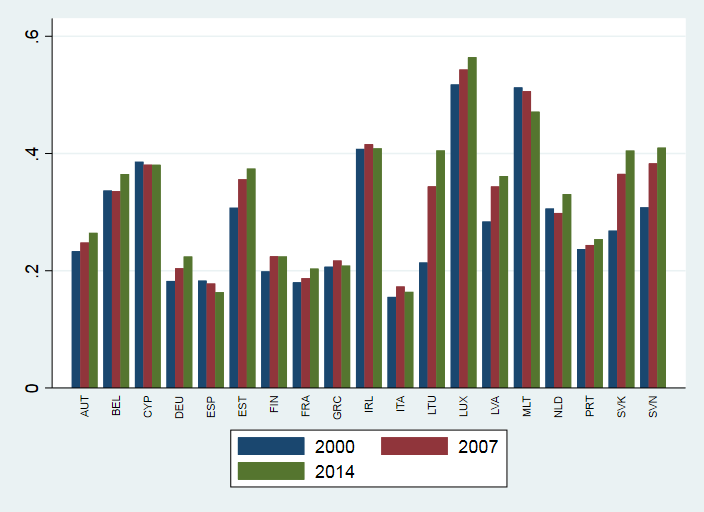
\includegraphics[width=5.0in, height=3.5in]{Graph_ratioimp_WIOD_2000_2014_ze}\\
\floatfoot{Source: WIOD}.
\end{tabular}
\label{fig:ratioimptemp_ze}
\end{figure}


\begin{figure}[!h]
\centering
\caption{\footnotesize{\textbf{Evolution of the intensity of import in household consumption}}}
\begin{tabular}{c}
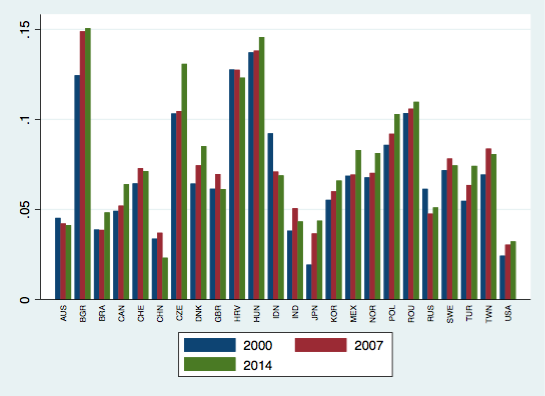
\includegraphics[width=5.0in, height=3.5in]{Graph_ratioimp_WIOD_2000_2014}\\
\floatfoot{Source: WIOD}.
\end{tabular}
\label{fig:ratioimptemp}
\end{figure}


\subsection{Domestic consumer prices reactions to changes in import prices}
In this section, we evaluate how domestic consumer prices react to changes in prices of imported intermediate and final goods, the latters being caused by exchange rate fluctuations. 
We are interested in (\textit{i}) the direct effect of global inflationary shocks, defined as the share of imported final and intermediate goods in domestic consumption (i.e. the import intensity in domestic consumption defined in Section \ref{subsec:intensity}) and (\textit{ii}) the total effect. The latter depends both on the direct effect and on the additional transmission of lower domestic input prices to other sectors of the domestic economy and to other countries which occurs during subsequent production cycles. 
\paragraph{How much of domestic consumer prices' reactions to changes in import prices is explained by the direct effect?}

Figure \ref{fig:ratiodir} depicts how much of the total impact of a change in import prices is explained by the import intensity of household consumption. In other words, Figure \ref{fig:ratiodir} represents the ratio of the direct effect to the total effect.
In all countries except Australia, Canada, China and Russia, the direct effect accounts for more than half of the total impact in 2014. In five economies (India, Indonesia, Luxembourg, Mexico and Turkey), the direct effect explains more than 80$\%$ of the reaction of domestic consumer prices to changes in import prices, which suggests that these countries do not provide much intermediate goods to their partners. For the whole cross-section, the coefficient of correlation between the total and the direct effect is close to 95$\%$ in 2014.

\begin{figure}[!h]
\centering
\caption{\footnotesize{\textbf{Ratio of direct to total effect of domestic consumer prices reactions to changes in import prices}}}
\begin{tabular}{c}
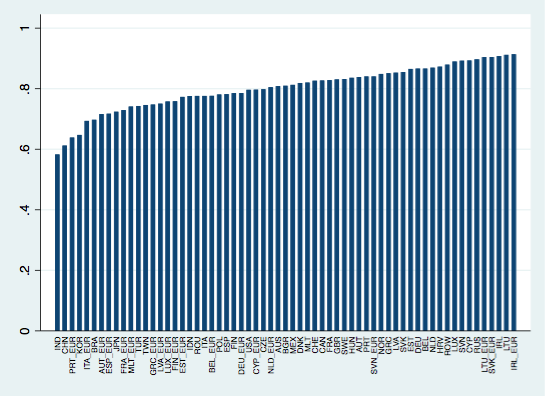
\includegraphics[width=5.0in, height=3.5in]{Graph_ratiodir_WIOD_2014}\\
\floatfoot{Source: WIOD, 2014}.
\end{tabular}
\label{fig:ratiodir}
\end{figure}


\paragraph{Is the import intensity of consumption a good predictor of domestic consumer prices reactions to changes in import price?}
To investigate whether the import intensity of consumption is a good predictor of domestic consumer prices reactions to changes in import price, we run the cross-section following regression (Equation \ref{eq:eq7}). 

 \begin{eqnarray}
{S^{HC}}=\beta  I + c +\varepsilon
\label{eq:eq7}
 \end{eqnarray}
 with ${S^{HC}}$ the vector of average impact of the devaluation shock on consumer prices ($\overline{s_{i}^{HC}}$), for each country $i$, defined in Equation \ref{eq:eq6} and $I$ the vector of country-specific import intensity of consumption.
 
Figure \ref{fig:ratiodir} depicts the relationship between the import intensity of consumption and the elasticity of consumer prices to an exchange rate shock.

\begin{figure}[!h]
\centering
\caption{\footnotesize{\textbf{Consumer prices elasticity to an exchange rate shock}}}
\begin{tabular}{c}
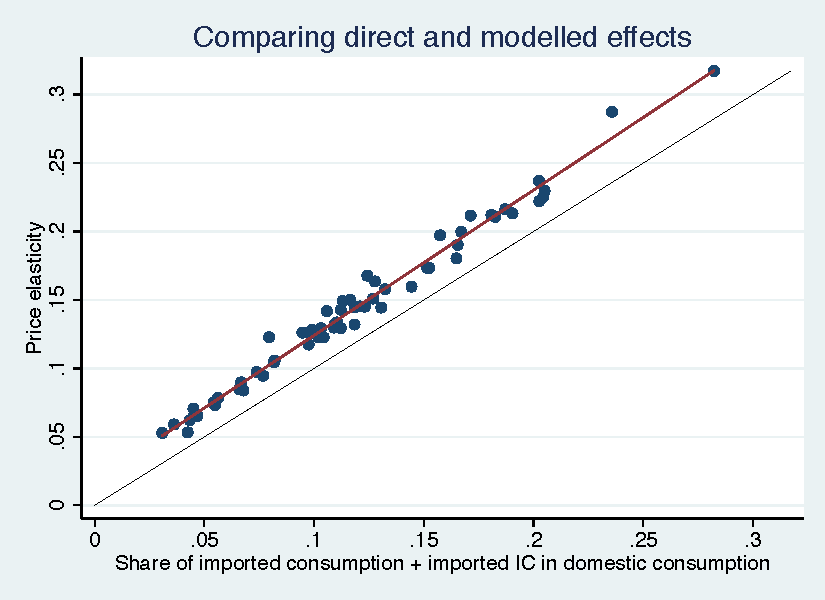
\includegraphics[width=5.0in, height=3.5in]{graph_2014_WIOD_HC}\\
\floatfoot{Source: WIOD, 2014. \\
The estimate corresponds to ${S^{HC}}=1.15 I + 0.04$ for 2014. Coefficients are significant at 1$\%$. Adjusted R2=0.89 A VÉRIFIER}
\end{tabular}
\label{fig:ratiodir}
\end{figure}

 

\section{The impact of exchange rates fluctuations on the main components of consumer prices}
\label{sec:prixconsosecteur}


\section{Conclusion}
\label{sec:ccl}
Real integration through the supply chain matters for domestic price dynamics in the euro area.

\newpage
\bibliography{PapiertransmissiondeschocsenVA}

\end{document}